


\begin{frame}[noframenumbering]
	\titlepage
\end{frame}


\begin{frame}{Биномиальное дерево}
	\textbf{Биномиальное дерево} \textit{(binomial tree)} $B_k$ представляет собой рекурсивно определенное упорядоченное дерево:
	\begin{enumerate}
		\item Биномиальное дерево $B_0$ состоит из одного узла.
		\item Биномиальное дерево $B_k$ состоит из двух биномиальных деревьев $B_{k−1}$,
		связанных вместе: корень одного из них является крайним левым дочерним узлом корня второго дерева.
	\end{enumerate}
\end{frame}

\begin{frame}{Биномиальное дерево} 
	\begin{figure}
		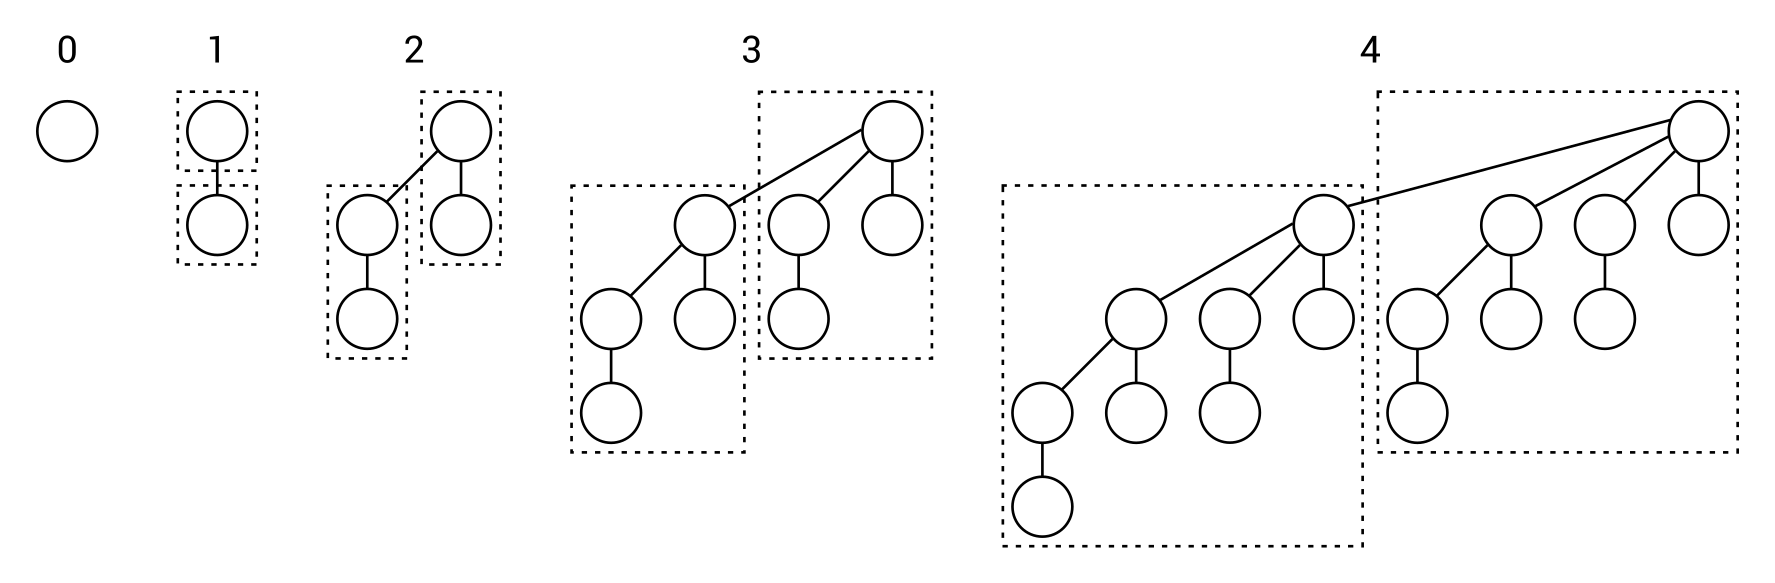
\includegraphics[width=0.9\linewidth]{images/binom-trees.png}
		\caption{Биномиальные деревья}
	\end{figure}
\end{frame}


\begin{frame}{Свойства биномиальных деревьев}
	\begin{enumerate}
		\item имеет $\mathbf{2^k}$ узлов;
		\item имеет высоту \textbf{k};
		\item имеет ровно $\mathbf{\binom{k}{i}}$ узлов на глубине \textit{i = 0, 1,...,k};
		%\item имеет корень степени \textbf{k}; степень всех остальных вершин меньше степени корня биномиального
	%	дерева. Кроме того, если дочерние узлы корня пронумеровать слева направо числами 
		%\textit{k − 1, k − 2,..., 0,} то \textit{i}-й
	%	дочерний узел корня является корнем биномиального дерева $B_i$.
	\end{enumerate}
\end{frame}


\begin{frame}{Биномиальная пирамида}
	\textbf{Биномиальная пирамида} (binomial heap) представляет собой множество
	биномиальных деревьев, которые удовлетворяют следующим свойствам:
	\begin{enumerate}
		\item Каждое биномиальное дерево в \textbf{H} подчиняется \textbf{свойству неубывающей пирамиды}:
		ключ узла не меньше ключа его родительского узла. 
		Мы говорим, что такие деревья являются \textbf{упорядоченными в соответствии со свойством 
		неубывающей пирамиды}.
		\item Для любого неотрицательного целого \textbf{k} имеется не более одного биномиального дерева 
		\textbf{H}, чей корень имеет степень \textbf{k}.
	\end{enumerate}
\end{frame}

\begin{frame}{Биномиальная пирамида: рисунок}
	\begin{figure}
		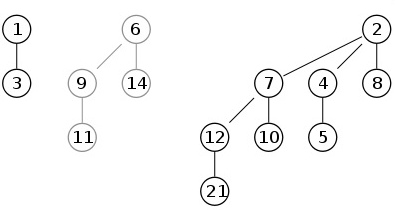
\includegraphics[width=0.6\linewidth]{images/binom-heap.png}
		\caption{Биномиальная пирамида}
	\end{figure}
	\begin{itemize}
		\item Минимальные элементы являются корнями деревьев.
	\end{itemize}
\end{frame}
	

\begin{frame}{Время выполнения операций}
	\centering
	\begin{tabular}{ |p{3cm}||p{3cm}|p{3cm}|  }
		\hline \textbf{Процедура} & \textbf{Бинарная пирамида} (наихудший случай) & \textbf{Биномиальная	пирамида} (наихудший случай) \\
		\hline
		make         & $\Theta(1)$    &$\Theta(1)$     \\
		insert       & $\Theta(\lg n)$& $O(\lg n)$     \\
		minimum      & $\Theta(1)$    & $O(\lg n)$     \\
		extract\_min & $\Theta(\lg n)$& $\Theta(\lg n)$\\
		union        & $\Theta(n)$    & $\Omega(\lg n)$\\
		decrease\_key& $\Theta(\lg n)$& $\Theta(\lg n)$\\
		delete       & $\Theta(\lg n)$& $\Theta(\lg n)$\\
		\hline
	\end{tabular}
\end{frame}

\begin{frame}{Создание новой биномиальной пирамиды}
	\begin{itemize}
		\item Для создания биномиальной пирамиды процедура \textbf{make}
		просто выделяет память и возвращает пустой объект \textbf{H}.
		\item Время работы этой процедуры составляет $\Theta(1)$.
	\end{itemize}
\end{frame}

\begin{frame}{Поиск минимального ключа}
	\begin{itemize}
		\item Минимальный ключ должен находиться в корне одного из деревьев.
		\item Для поиска минимума надо обойти корни всех деревьев. Их число не превышает $\lg n + 1$.
		\item Поскольку надо проверитьне более $\lg n + 1$ корней, время работы процедуры
		\textbf{minimum} составляет $O(\lg n)$.
	\end{itemize}

	\begin{figure}
		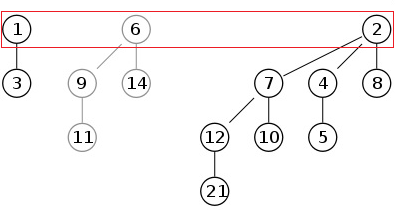
\includegraphics[width=0.6\linewidth]{images/binom-heap-min.png}
	\end{figure}
\end{frame}

\begin{frame}{Слияние двух биномиальных пирамид}
	Процедура \textbf{union} имеет две фазы:
	\begin{itemize}
		\item объединяем списки корней биномиальных пирамид $H_1$ и $H_2$ в единый связанный список H, который
		отсортирован по степеням корней в монотонно возрастающем порядке.
		\item постепенно объединяем мелкие биномиальные деревья в более крупные.
		В получившемся списке могут встречаться пары соседних вершин одинаковой степени. 
		Поэтому мы начинаем соединять деревья равной степени и делаем это до тех пор, 
		пока деревьев одинаковой степени не останется. Операция выполняется за $\Omega(\lg n)$.
	\end{itemize}
\end{frame}

\begin{frame}{Слияние двух биномиальных пирамид}
	\begin{figure}
		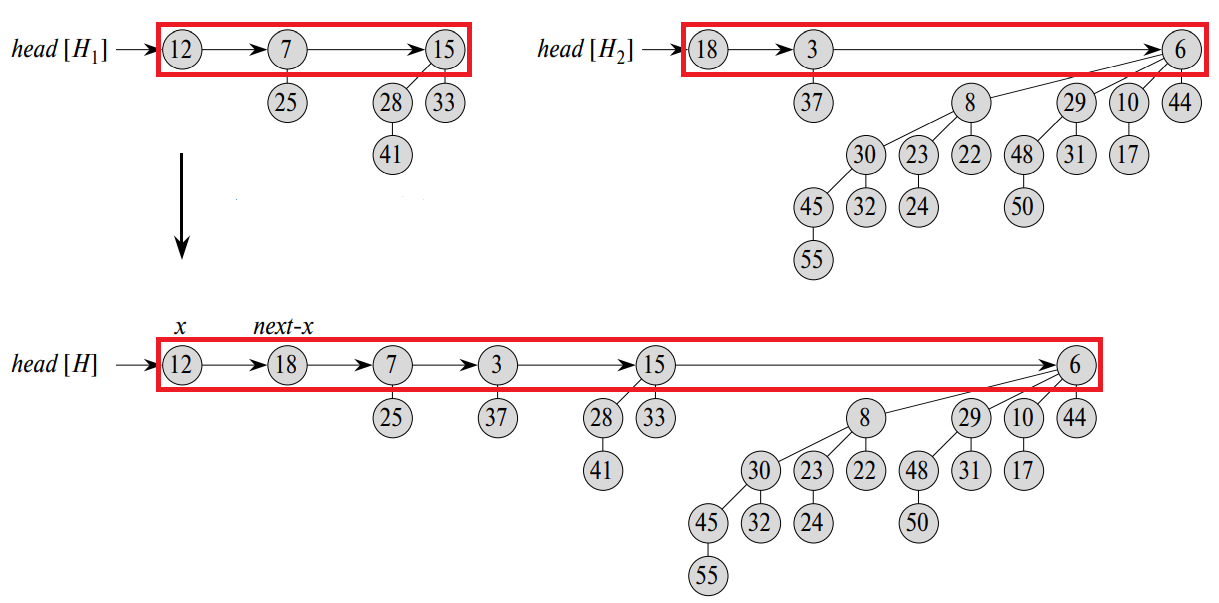
\includegraphics[width=0.9\linewidth]{images/binom-heap-union0.png}
	\end{figure}
\end{frame}

\begin{frame}{Слияние двух биномиальных пирамид}
	\begin{figure}
		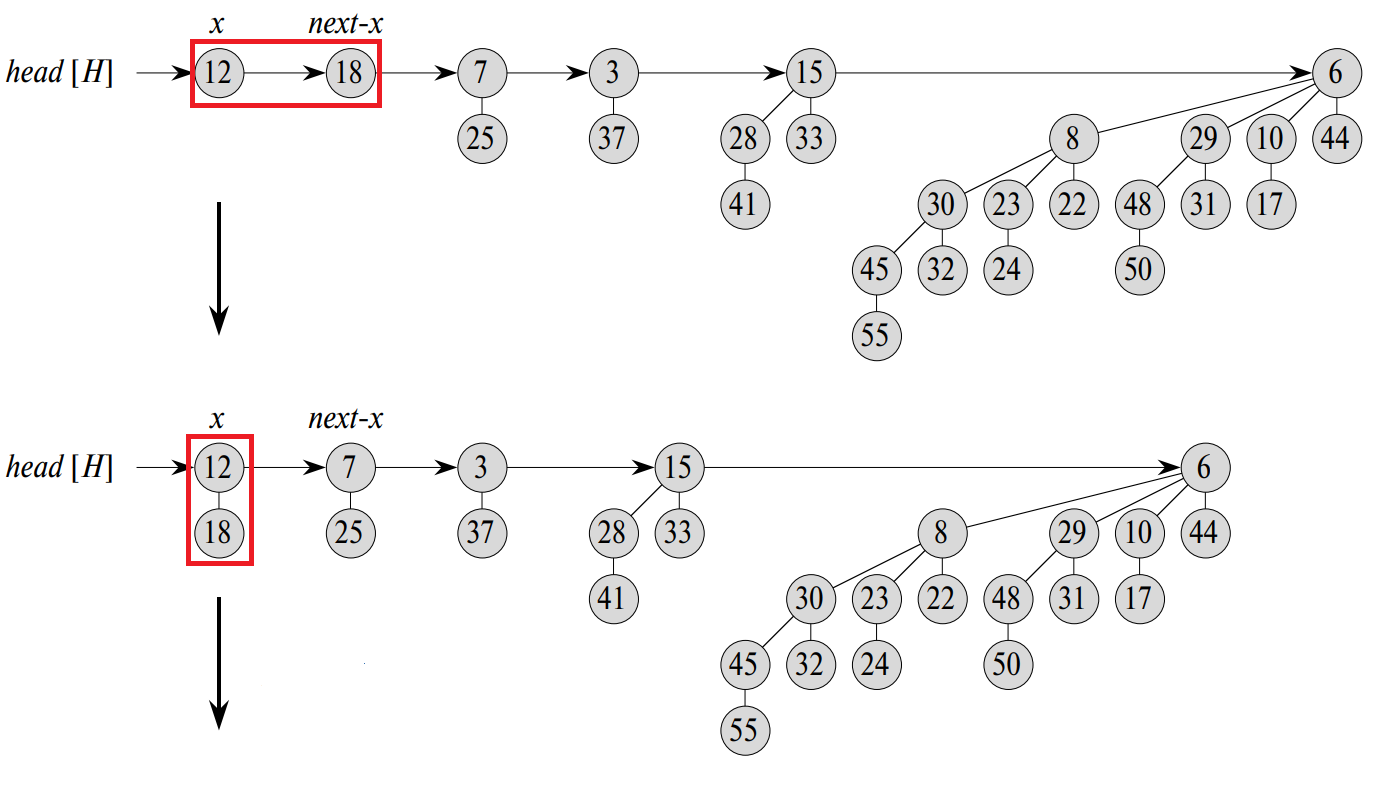
\includegraphics[width=0.9\linewidth]{images/binom-heap-union1.png}
	\end{figure}
\end{frame}

\begin{frame}{Слияние двух биномиальных пирамид}
	\begin{figure}
		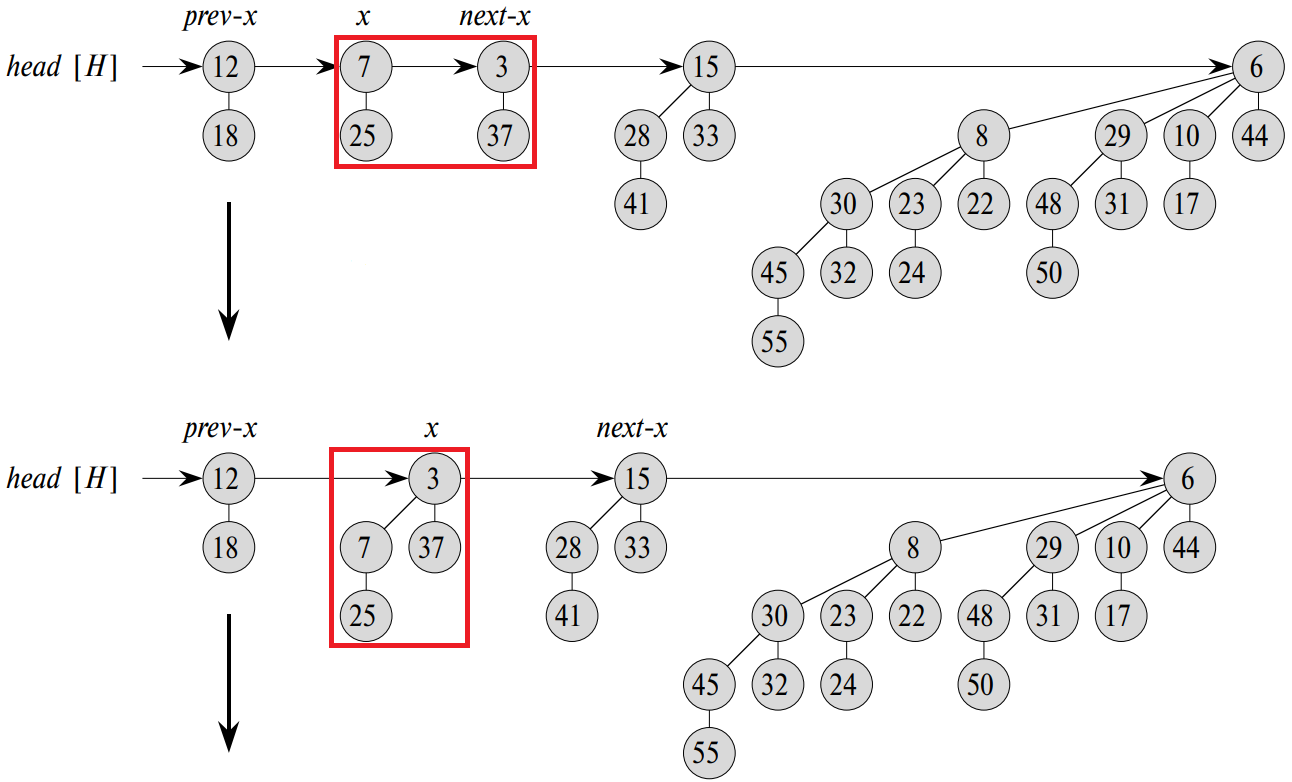
\includegraphics[width=0.85\linewidth]{images/binom-heap-union2.png}
	\end{figure}
\end{frame}

\begin{frame}{Слияние двух биномиальных пирамид}
	\begin{figure}
		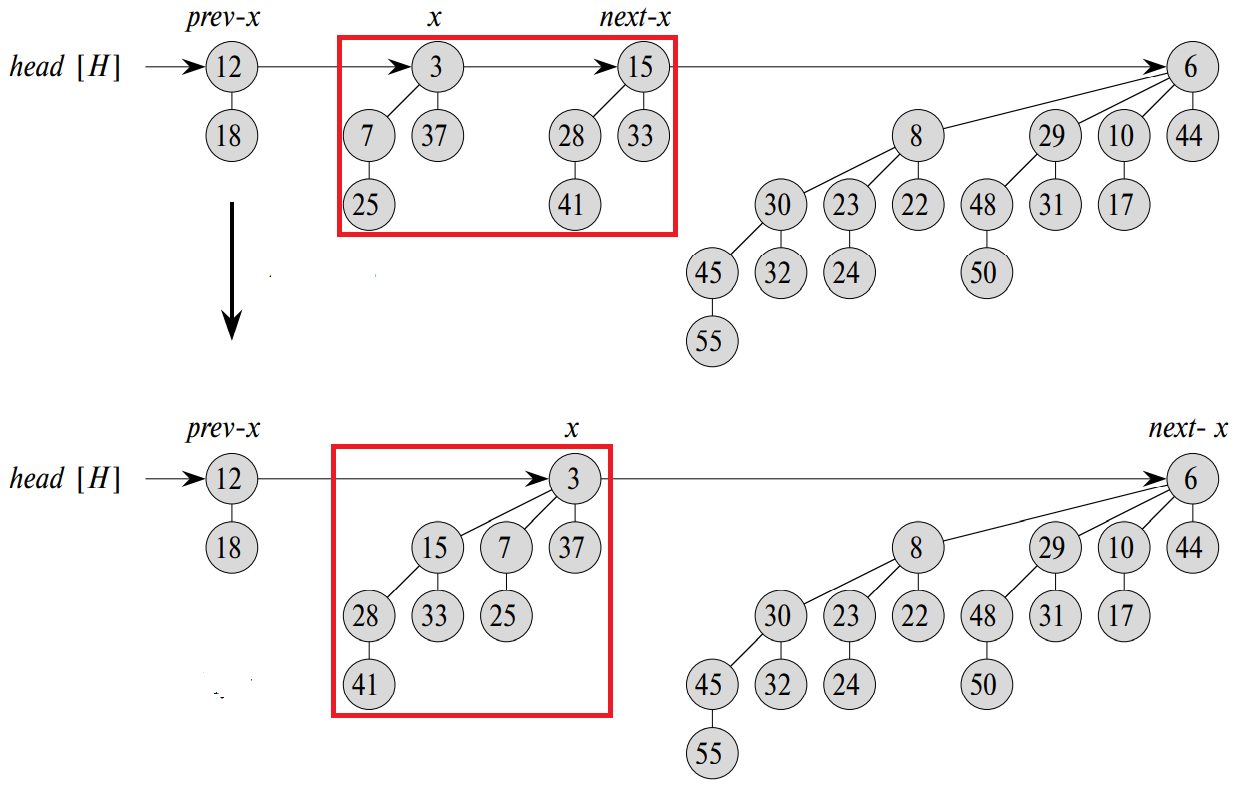
\includegraphics[width=0.8\linewidth]{images/binom-heap-union3.png}
	\end{figure}
\end{frame}

\begin{frame}{Вставка узла}
	Процедура \textbf{insert}:
	\begin{itemize}
		\item создает биномиальную пирамиду \textbf{H'} с одним элементом за время $O(1)$.
		\item объединяет ее с биномиальной пирамидой \textbf{H}, содержащей n узлов, за время $O(\lg n)$. 
	\end{itemize}
	Вызов \textbf{union} должен освободить память, выделенную для временной биномиальной пирамиды \textbf{H}.
\end{frame}

\begin{frame}{Извлечение вершины с минимальным ключом}
	Процедура \textbf{extract\_min}:
	\begin{enumerate}
		\item находим элемент при помощи \textbf{minimum}.
		\item удаляем его из корневого списка. Из перевернутого списка его детей делаем 
		корневой список для новой кучи $H_1$.
		\item объединяем исходную кучу с $H_1$.
	\end{enumerate}
	Сложность $\Theta(\lg n)$.
\end{frame}

\begin{frame}{Извлечение вершины с минимальным ключом}
	\begin{figure}
		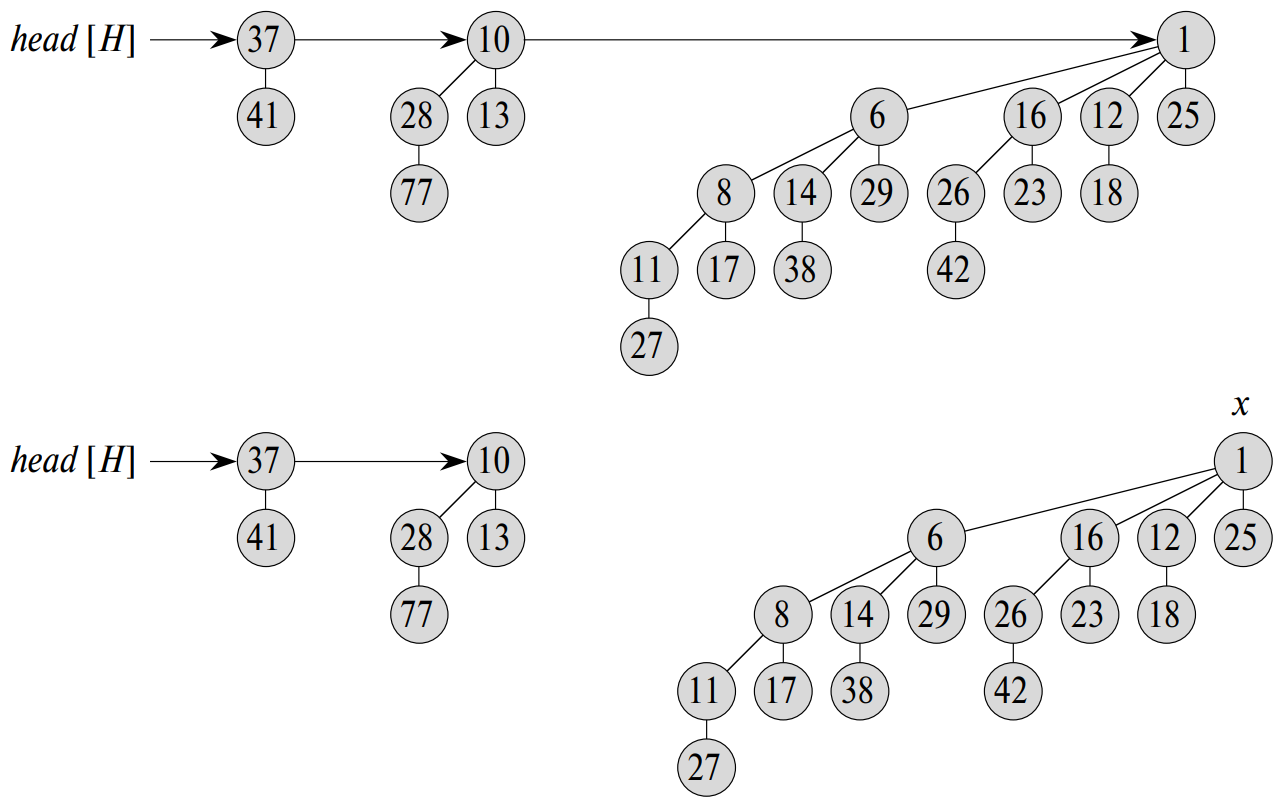
\includegraphics[width=0.8\linewidth]{images/binom-heap-extract-min0.png}
	\end{figure}
\end{frame}

\begin{frame}{Извлечение вершины с минимальным ключом}
	\begin{figure}
		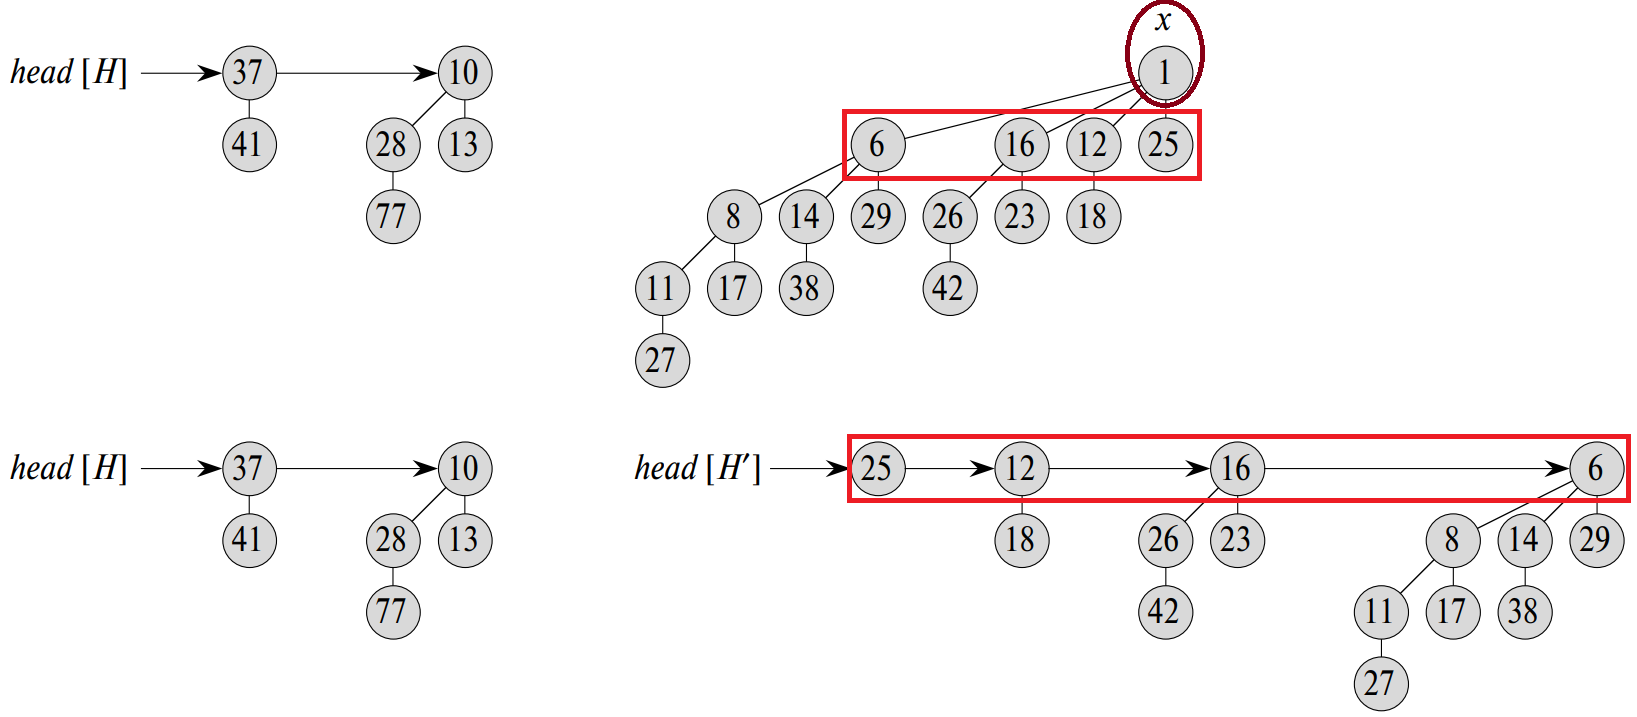
\includegraphics[width=1\linewidth]{images/binom-heap-extract-min1.png}
	\end{figure}
\end{frame}

\begin{frame}{Извлечение вершины с минимальным ключом}
	\begin{figure}
		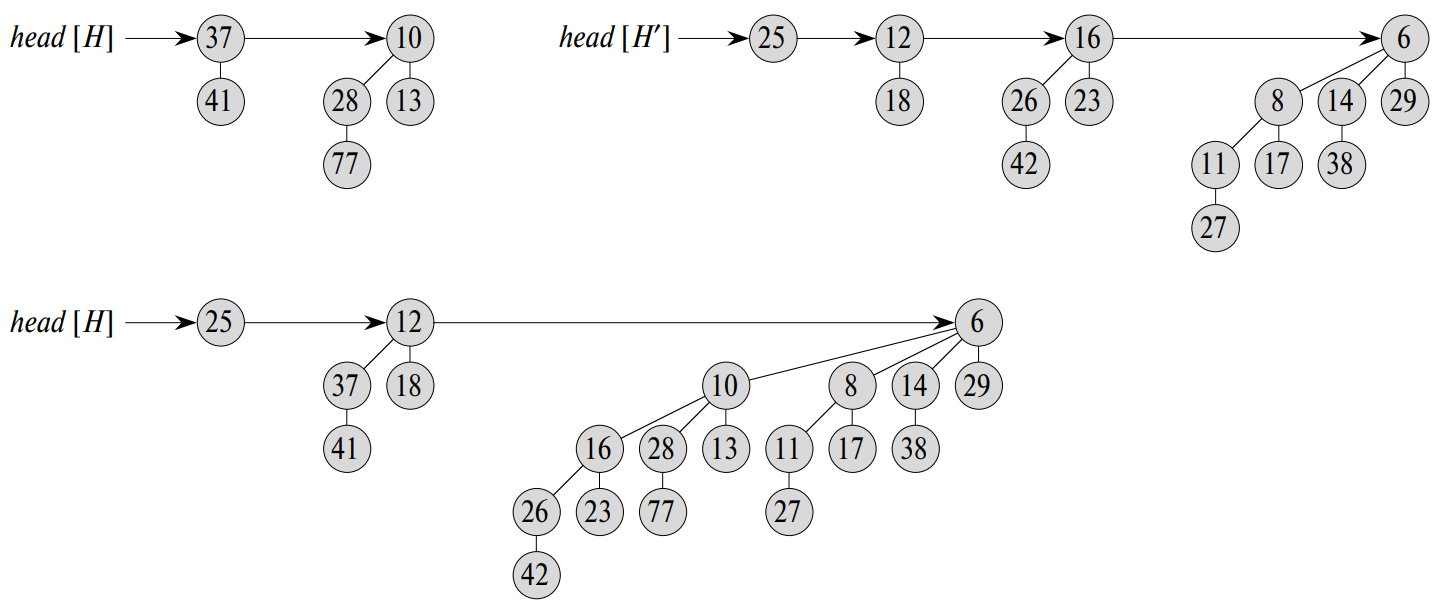
\includegraphics[width=1\linewidth]{images/binom-heap-extract-min2.png}
	\end{figure}
\end{frame}

\begin{frame}{Уменьшение ключа}
	Процедура \textbf{decrease\_key}:
	\begin{itemize}
		\item уменьшает значение ключа узла \textbf{x} в 
	биномиальной пирамиде \textbf{H}, присваивая ему новое значение \textbf{k}.
		\item В случае, если \textbf{k} превышает текущий ключ \textbf{x}, процедура сообщает об ошибке.
	\end{itemize}
\end{frame}
	
\begin{frame}{Уменьшение ключа}
	\begin{figure}
		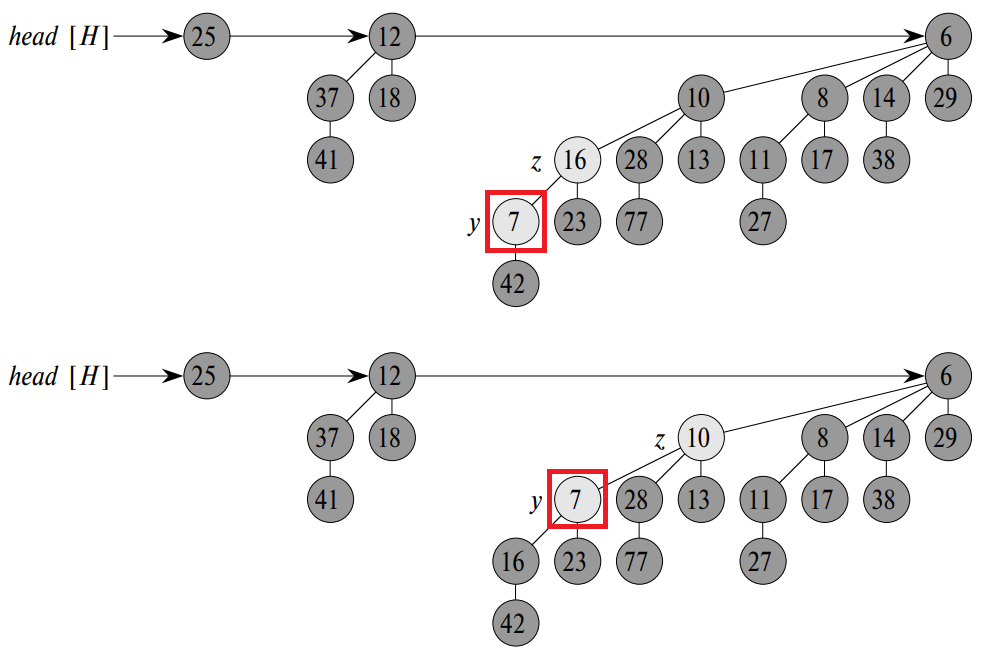
\includegraphics[width=0.8\linewidth]{images/binom-heap-decrease0.png}
	\end{figure}
\end{frame}
		
\begin{frame}{Уменьшение ключа}
	\begin{figure}
		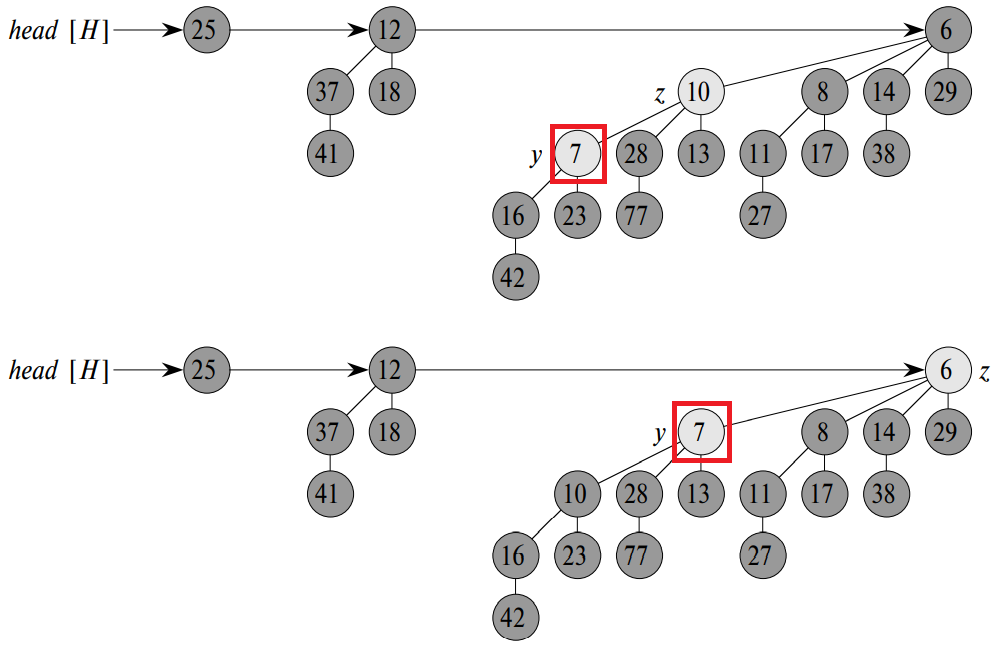
\includegraphics[width=0.8\linewidth]{images/binom-heap-decrease1.png}
	\end{figure}
\end{frame}

\begin{frame}{Удаление ключа}
	Операция \textbf{delete} сводится к \textbf{decrease\_key} и \textbf{extract\_min}:
	\begin{itemize}
		\item сначала нужно уменьшить ключ до минимально возможного значения, 
		а затем извлечь вершину с минимальным ключом.
		\item узел всплывает вверх, откуда и удаляется \textbf{extract\_min}.
	\end{itemize}
	Процедура выполняется за время $\Theta(\lg n)$.
\end{frame}

\begin{frame}{Использование}
	\begin{enumerate}
		\item Применяется для реализации \textbf{очереди с приоритетом}.
		\item Так же подходит для создания lock-free concurent queue:
		\par
		\textit{Gavin Lowe. "Lock-Free Concurrent Binomial Heaps", 2018}
	\end{enumerate}
\end{frame}

\begin{frame}{Comparison concurrent priority queue implementations}
	\begin{figure}
		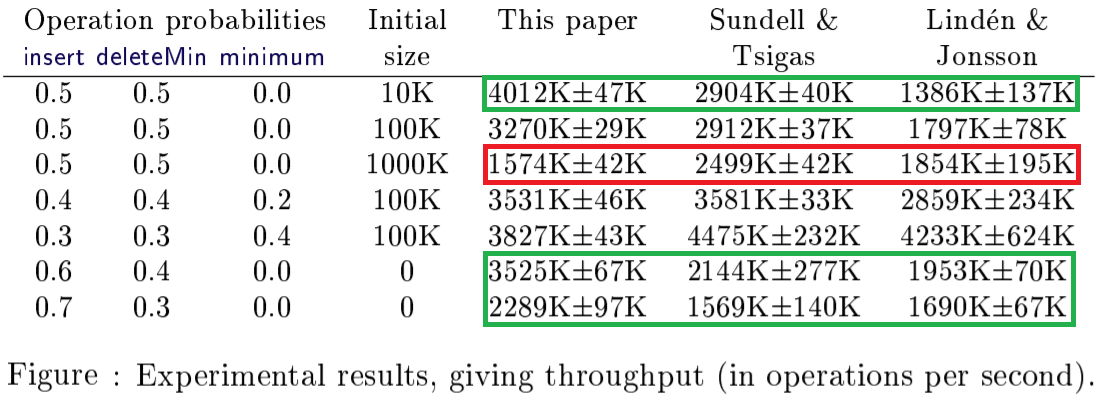
\includegraphics[width=0.8\linewidth]{images/result-bench.png}
	\end{figure}
	\begin{itemize}
		\item 64 threads, 2.1GHz Intel(R) Xeon(R) E5-2683 CPUs with 256GB of RAM
		\item two million randomly chosen operations
		\item 10 executions and $95\%$ condence intervals.
	\end{itemize}
\end{frame}